\documentclass[a4paper,english,twoside]{scrreprt}
  \usepackage[utf8]{inputenc}
  \usepackage{babel,geometry,amsmath}
  \usepackage{graphicx,afterpage,float}
  \usepackage[nottoc,numbib]{tocbibind}
  \usepackage[hidelinks]{hyperref}
 % \usepackage[title,titletoc]{appendix}
  \usepackage{fancyhdr}
  \setlength{\headheight}{13.6pt}
  \pagestyle{fancy}
  \renewcommand{\chaptermark}[1]{ \markboth{#1}{} }
  \renewcommand{\sectionmark}[1]{ \markright{#1}{} }

  \fancyhf{}
  \fancyfoot[LO,RE]{\thepage}
  \renewcommand{\footrulewidth}{0.4pt}
  %\renewcommand{\headrulewidth}{0pt} 
  \fancyhead[RE]{\textit{ \nouppercase{\leftmark}} }
  \fancyhead[LO]{\textit{ \nouppercase{\rightmark}} }

  \fancypagestyle{plain}{ %
    \fancyhf{} % remove everything
    \fancyfoot[LO,RE]{\thepage}
    \renewcommand{\headrulewidth}{0pt} % remove lines as well
    %\renewcommand{\footrulewidth}{0pt}
  }
  \renewcommand{\chapterheadstartvskip}{\vspace *{0.1\baselineskip }}
  \makeatletter
\g@addto@macro\appendix{%
  \renewcommand*{\chapterformat}{%
    {\chapapp\nobreakspace\thechapter\autodot\enskip}%
  }
  \renewcommand*{\chaptermarkformat}{%
    {\chapapp\nobreakspace\thechapter\autodot\enskip}%
  }
  \let\oldaddcontentsline\addcontentsline
  \newcommand\hackedaddcontentsline[3]{\oldaddcontentsline{#1}{#2}{\chapapp\nobreakspace#3}}
  \let\oldchapter\chapter
  \renewcommand*\chapter[1]{%
    \let\addcontentsline\hackedaddcontentsline%
    \oldchapter{#1}%
    \let\addcontentsline\oldaddcontentsline%
  }
}
\makeatother

\begin{document}

  \begin{titlepage}

	\begin{center}~
		\\[5cm]

		
\includegraphics[width=0.4\textwidth]{./img/logontnu}~
		\\[0.3cm]
		\textsc{ Department of Electronics and Telecommunications}~
		\\[2cm]

		{ \huge \bfseries TTT4212 RF/Microwave Design and Measurement Techniques \\[0.5cm]
		Term Project Fall 2014 }~
		\\[1.5cm]
		

		{ \LARGE J\o rn Fr\o ysa, Helge Langen, Lars-Arne Larsen}
	\end{center}


\end{titlepage}

  \clearpage
  \setcounter{page}{1}

  \chapter*{Abstract}
\addcontentsline{toc}{chapter}{Abstract}
This report describes the process of designing, building and verifying an RF power amplifier for the 2.4 GHz$\pm$50MHz frequency band. The Cree CGH40010F GaN transistor is used as the active device. The circuit is built on standard FR-4 substrate. The circuit is designed and simulated in the Keysight ADS software suite, then built and measured using standard RF measurement instruments such as a network analyzer and spectrum analyzer.

The resulting amplifier was measured to have a small-signal gain of 14dB at the center frequency of 2.4 GHz, however, the gain diminished rapidly towards the lower end of the operating band at 2.35 GHz. Also the large-signal power gain and power added efficiency showed poorer performance at the lower end of the operating band. At 2.4 GHz, the large-signal gain with an input signal of 27dBm was measured to 10dB with a power-added efficiency of 35\% . Third-order intermodulation distortion was measured to -22dBc at a peak output power of 38dBm with a two-tone input signal with 5Mhz spacing.

  \clearpage

  \tableofcontents	
  \clearpage

  \chapter{Introduction}
In the course TTT4212 RF/Microwave design and measurement techniques at NTNU, the students are given the task of designing, building and verifying the performance parameters of an RF power amplifier. The amplifier should fulfill the following requirements and design restrictions:

\begin{itemize}
	\item Center operating frequency of 2.4 GHz
	\item Based on the Cree CGH40010F GaN transistor
	\item Drain voltage biased at 28V
	\item Gate voltage biased at -3.0V or higher
	\item The amplifier should be unconditionally stable
	\item Small-signal bandwidth of at least 100 Mhz
	\item Small-signal gain of at least 13dB throughout the bandwidth
	\item Output power of at least 39dBm with a single-tone input power of 27dBm
	\item Some geometrical restrictions for the board layout are given to make the amplifier fit on a standardized heatsink, to avoid the added time, cost and complications of manufacturing customized heatsinks for each group of students.
\end{itemize}
The power added efficiency (with a single-tone input signal at 27dBm) and intermodulation distortion (for a two-tone signal with 5 Mhz spacing and a peak output power of 38 dBm) should also be measured, however, no requirements for these performance parameters are given, and it will be up to the group members’ to decide which parameters to focus on optimizing (as long as the requirement specification is fulfilled.

The circuit shall be designed and simulated in the Keysight Advanced Design System (ADS) software suite for computer-aided design (CAD) and simulation of microwave circuits, and all performance parameters shall be verified to be within the requirement specification before proceeding to making a board layout (also in ADS), generating the Gerber production files for having the printed circuit board manufactured, and then building the amplifier and doing real world measurements at the lab.

  \chapter{Theory}

\section{Bias point and class operation}
The bias point, or working point, of an amplifier determines which class the amplifier is, which in turn tells us something about the amplifiers efficiency, linearity and quiescent current. There is a wide variety of classes, the most common being class A, AB, B and C. 
Class A amplifiers have the highest quiescent current, the best linearity and the lowest efficiency (maximum theoretical efficiency of 50\% ). 
Class B amplifiers have no quiescent current, maximum theoretical efficiency of 78\% , but only conducts the positive half-period of a signal. 
Class AB is a hybrid between class A and B, sacrificing some of the efficiency of the class B amplifier, but gaining some of the linearity of the class A. 
Class C amplifiers are the most efficient of the four, having a maximum theoretical efficiency of almost 90\% . But they conduct for less than 50\%  of the signal cycle, typically they only conduct for a third of the cycle or less.
If the input signal of the amplifier is sufficiently small, one can bias the amplifier as an AB class, thus reducing quiescent current while still have class A operation in terms of linearity.

Once a class has been chosen, the bias point can be determined by examining the I-V characteristics of the transistor. By drawing a loadline going from the drain-source voltage on the X axis, to the drain saturation current on the Y axis, we get a linear line crossing the different gate-source voltage curves. See figure~\ref{fig:fig_Load_line}. By choosing a bias point along this linear curve, we can predict both quiescent current and voltage. The bias point for a class A amplifier will approximately be at Vds/2. The closer you move the bias point towards the maximum Vds voltage, the lower the class you get. This is because the loadline represents the current through and voltage across the transistors equivalent resistor.

\begin{figure}[H]
	  \centering
	  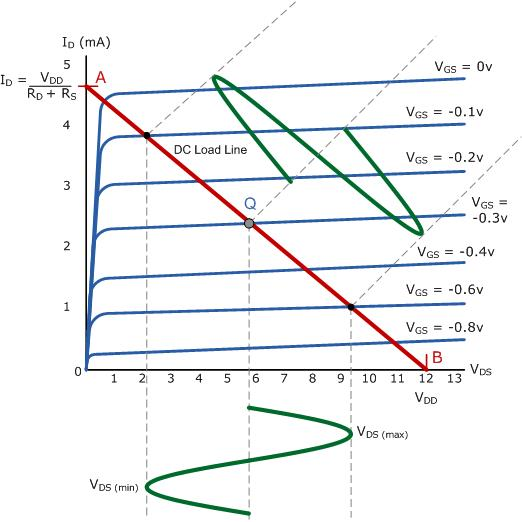
\includegraphics[width=0.75\textwidth]{img/Load_line_graphics}
	  \caption{Load line for class A amplifier}
	  \label{fig:fig_Load_line}
\end{figure}

\section{Efficiency}
There are several ways of expressing amplifier efficiency, the most common in the RF community being power added efficiency (PAE). PAE takes into account both the DC to RF power conversion, as well as the RF power delivered into the input of the device.

\begin{equation}
	PAE=\frac{P_{RFout}-P_{RFin}}{P_{DC}}=\frac{P_{RFout}-P_{RFin}}{V_{DC} \times I_{DC}} 
\end{equation}
By subtracting the power added to the input of the device from the output power, we get a better indication of the actual DC to RF power conversion. For low gain amplifiers the input power can be substantial and using drain efficiency (which does not take input power into consideration), will in these cases give a falsely high efficiency.
\section{Linearity}
Linearity is an important factor to consider when designing an amplifier. A linear amplifier will amplify a small input signal and a large input signal by the same amount, but better linearity often comes at the cost of efficiency, as the quiescent current must be increased. To better see the linearity of a transistor one can plot the drain current as a function of the gate-source voltage. This will produce a characteristic plot which shows how linear the transistor is for certain regions of the input signal.
\begin{figure}[H]
	  \centering
	  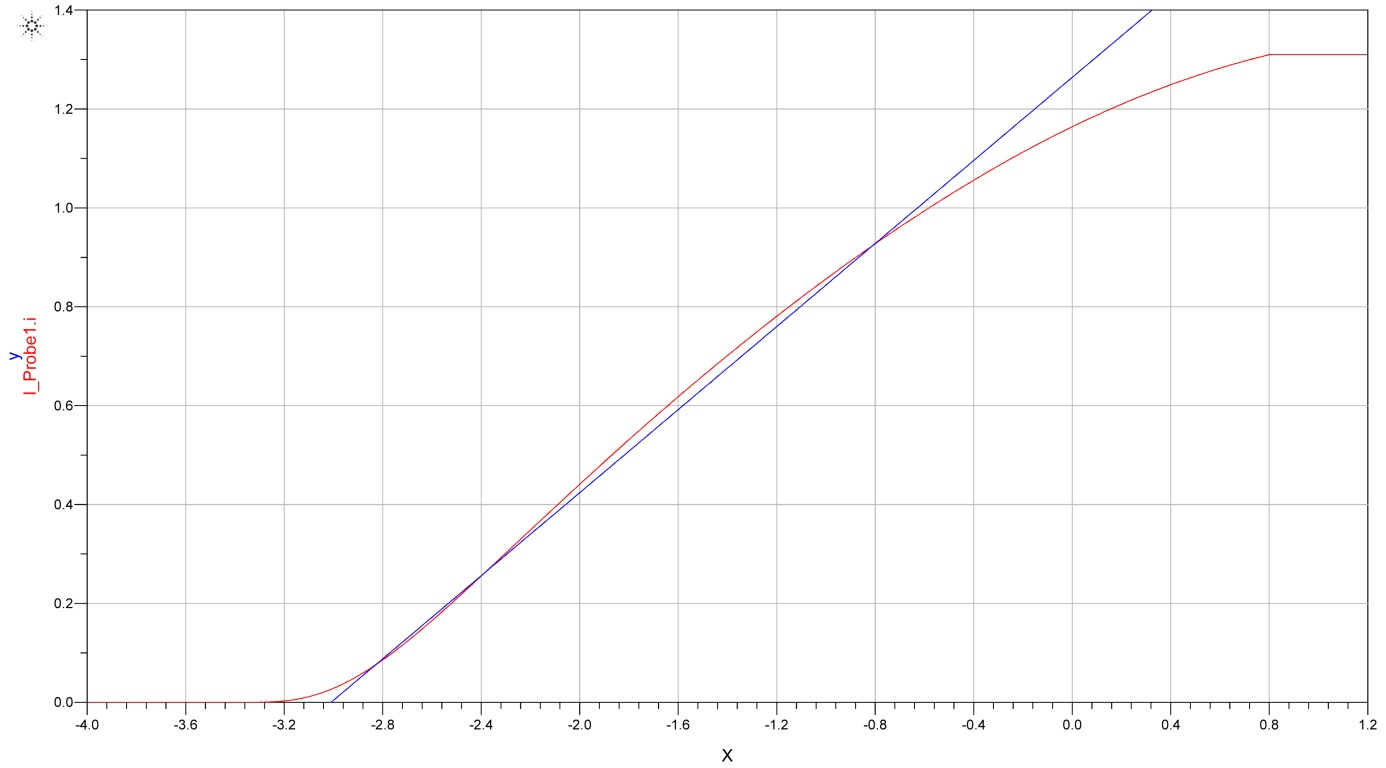
\includegraphics[width=0.75\textwidth]{img/Linearity_curve}
	  \caption{Drain current plotted vs gate-source voltage (shown in red). The blue line is a linear curve, making it easier to see the linearity of the device}
	  \label{fig:fig_Linearity_line}
\end{figure}
We can see in figure~\ref{fig:fig_Linearity_line} the most linear area for this device approximately lie between $-2.8V$ and $-2.4V$. Biasing the transistor for $-2.6V$ would offer the most linear response as long as the amplitude of the input signal does not exceed $0.2V$ in the negative half period, which would drive the gate-source voltage below $-2.8$ volts and into cut-off. 
\section{S-parameters}
S-parameters, or scattering parameters, are a set of 4 parameters which describe a systems electrical behavior. When referring to two-port amplifiers we use the parameters $S_{11},\, S_{12},\, S_{21}$ and $S_{22}$.
\begin{figure}[H]
	  \centering
	  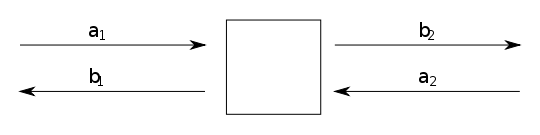
\includegraphics[width=0.75\textwidth]{img/S_parameter_image}
	  \caption{two-port signals for s-parameters}
	  \label{fig:fig_sparam_vis}
\end{figure}
 $S_{11}$ refers to the reflection of a input signal in $a_1$, returning back to the source through $b_1$, $S_{12}$ refers to the reverse voltage gain, $S_{21}$ refers to the forward voltage gain and $S_{22}$ refers to the reflection of the output signal in b2 back through $a_2$.
 The relationship between incident power, reflected power and the S-parameter matrix is given by the equation:
 \begin{equation}
	\begin{bmatrix}
	b_1\\
	b_2
	\end{bmatrix}
	=
	\begin{bmatrix}
	S_{11} & S_{12}\\
	S_{21} & S_{22}
	\end{bmatrix}
	\times
	\begin{bmatrix}
	a_1\\
	a_2
	\end{bmatrix}
 \end{equation}

\section{Stability}
Amplifier stability refers to the amplifiers tendency to oscillate, which is something we strive to prevent. Oscillations occure when the "reflected" value of an incident voltage (at either input or output) is larger than 1.
\begin{figure}[H]
	  \centering
	  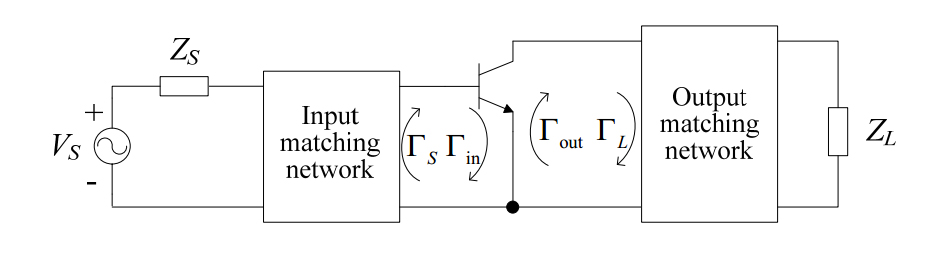
\includegraphics[width=0.75\textwidth]{img/Reflection_example}
	  \caption{reflections of an amplifiers circuit}
	  \label{fig:fig_reflection_ex}
\end{figure}
In Figure~\ref{fig:fig_reflection_ex} the $\Gamma_s$ refers to the reflection of the returning signal to the source, $\Gamma_{in}$ is the reflection of the input, $\Gamma_{out}$ is the reflection of returning signals at the output and $\Gamma_L$ is the reflection of signals to the load. If the input and output matching networks are passive, then $|\Gamma_s|<1$ and $|\Gamma_L|<1$. The circuit can be unstable if $|\Gamma_{in}|>1$ and $|\Gamma_{out}|>1$. 

By expressing $|\Gamma_{in}|$ and $|\Gamma_{out}|$ as functions of $\Gamma_L$  and $\Gamma_s$ respectively, in combination with the S-parameters, we can find an expression for a circle in the smith chart which represents the border between the region of stability and instability at input and output. These are called stability circles, and can tell us at what impedances the device is stable, or unstable.
There are two main measures of stability, the K-factor and the mu-factors:
\begin{equation}
K=\frac{1-|S_{11}|^2-|S_{22}|^2+|\nabla |^2}{2\times |S_{21}\times S_{12}|},\, \nabla =S_{11}\times S_{22}-S_{12}\times S_{21}
\end{equation}
The K-factor tells us whether or not the amplifier is stable for a specific frequency, which means we need to evaluate the K-factor from 0Hz (DC) to the highest frequency the amplifier can oscillate at. If K>1 the amplifier is stable for the specific frequency. If K>1 for all frequencies we say the amplifier is unconditionally stable, if there are frequencies where K<1, we say the amplifier is conditionally stable.  The K-factor tells us if the amplifier is stable, but not by how much. A larger value of K does not indicate a more stable amplifier. When designing an amplifier it is useful to know how stable our device is, so we can take variations in the manufacturing process into consideration. For this purpose we use the mu-factors:
\begin{equation}
\mu=\frac{1-|S_{11}|^2}{|S_{22}-\nabla \times S_{11}^*|+|S_{12}\times S_{21}|}>1
\end{equation}
\begin{equation}
\mu_{prime}=\frac{1-|S_{22}|^2}{|S_{11}-\nabla \times S_{22}^*|+|S_{12}\times S_{21}|}>1
\end{equation}
The mu-factors tell us the distance from the center of the smith chart, to the edge of the stability circle. Mu shows this distance for the output, while mu-prime shows the same for the input. If the value of the factor is above 1 the device is unconditionally stable for the given frequency, and the larger the values of the factors are the more stable a device is. This way we can add some margin to our amplifiers stability, to ensure it is stable after the manufacturing process.
\section{Quarter wave transformation}
For high frequency applications great care must be taken when designing the transmission lines on the PCB layout, as the wavelength of the signals are comparable to the lengths of the PCB traces. This causes the transmission lines to have significant capacitive or inductive effects on the signal, depending on the trace length. This allows us to create RLC circuits without the use of lumped components by strategically choosing the length, width and shape of each trace. A transmission line with a length equal to the signal wavelength will result in a $360^\circ$ phase-shift in the signal. Similarly a trace with a length equal to a quarter of the wavelength would result in a $90^\circ$ phase shift. If we have an open stub with a length equal to $^1/_4$ wavelength, the impedance at the open end of the stub would be infinite. The voltage at that point would be high, while the current would be zero. At the other end of the stub, the phase of the signal would have shifted  $90^\circ$, and the stub would appear to be a short circuit. This effect is highly frequency dependent, and the circuit can thusly be designed to only affect the signals of our choosing.
\section{Matching}
To affect stability, performance and efficiency matching networks are created at the amplifier input and output to adjust the impedance “seen” by the source and load. See figure~\ref{fig_reflection_ex}. For maximum power transfer, the output and input matching networks are matched to the characteristic impedance at the source and load, usually $50\Omega$ and sometimes $75\Omega$. For maximum gain or low noise the networks must be intentionally designed with mismatches compared to the characteristic impedances. By tweaking the networks matching, we can find a balance between the desired properties.

\section{Small signal vs large signal}
Small and large signal analysis is used to evaluate the amplifier design once a bias point has been chosen. When performing small signal analysis we use the chosen bias point, and look at the amplifiers response in the linear area of operation. Here we can assess the amplifiers gain, linearity and efficiency for signals well within the amplifiers capabilities.
When looking at large signal analysis on the other hand we use large input signals to drive the amplifier into compression, and the non-linear area of operation. Here we can find the 1 dB compression point, the input signal level at which the amplifiers amplification is reduced by 1 dB.

\section{Intermodulation distortion}
Intermodulation distortion (IMD) is found when performing a two tone test on a non-linear device. A linear amplifier would produce two tones at the same frequencies as the input signals but amplified in power. A non-linear device will create harmonics, and if subjected to a two-tone test it will also create signals which are the result of intermodulation (see figure~\ref{fig_distortion_vis}). As can be seen in the figure the intermodulation distortion components are caused by the summation (both additive and subtractive) of the harmonics of the two tones, creating distortion around the fundamental frequencies, as well as between the second and third harmonics.
\begin{figure}[H]
	  \centering
	  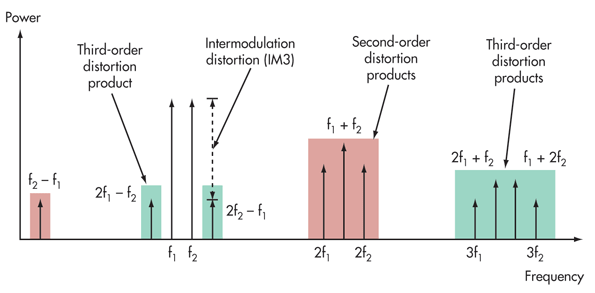
\includegraphics[width=0.75\textwidth]{img/Intermodulation_distortion}
	  \caption{Intermodulation distortion visualization}
	  \label{fig:fig_distortion_vis}
\end{figure}

  \chapter{Design of circuit}
  
  \section{DC Bias point at gate}

  We are using ADS to simulate the I-V characteristics of the CGH40010 transistor. ADS is providing a built-in design guide for this purpose. Figure~\ref{fig:fig_IV} shows the I-V characteristics, with drain current on the y-axis, drain voltage on the x-axis and curves for various gate voltages from -5 to -1 volts in 0.2 volts increments. Refering to figure 5.12 in \cite[p.~200]{AmpRobertson}, we choose to set a bias point at approximately 70\% of the maximum saturated drain current IDS, to achieve a good compromise between good linearity and high gain. We find this to be a gate voltage of about -1 volts.

  \begin{figure}[h]
	  \centering
	  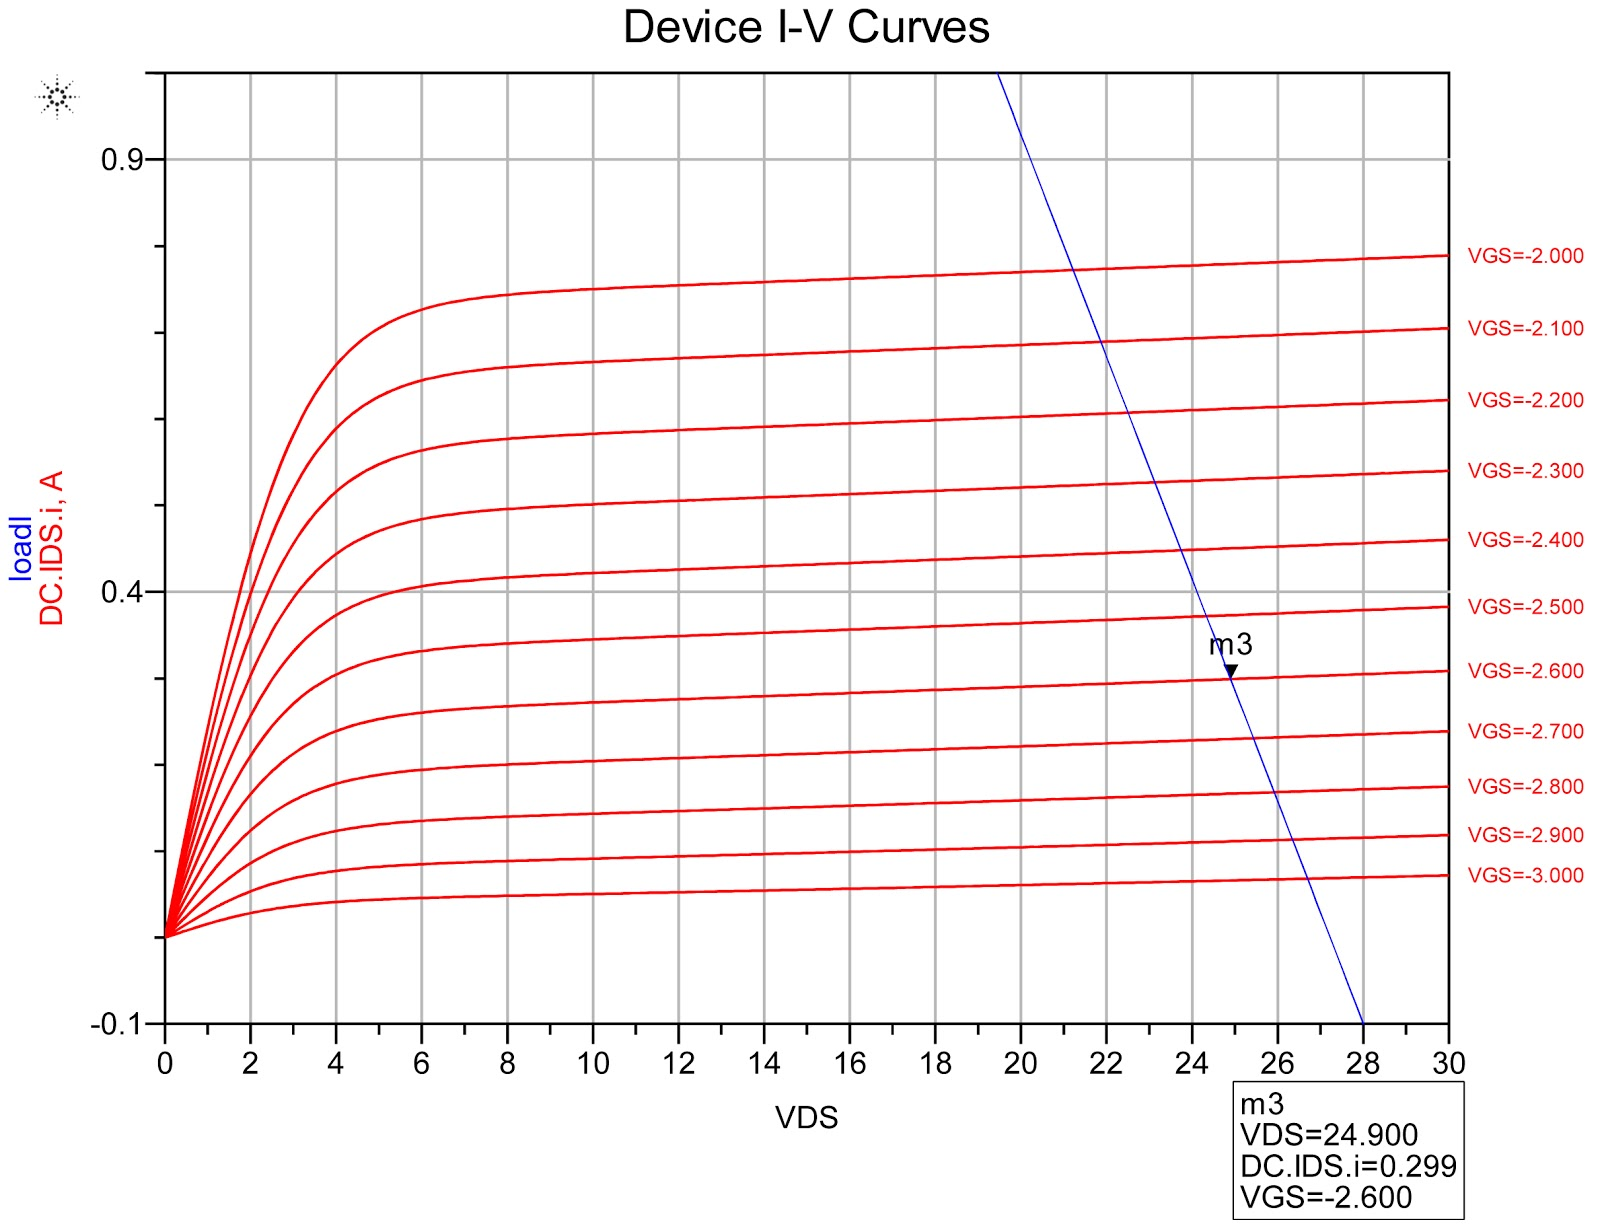
\includegraphics[width=0.75\textwidth]{img/01_IVCurve}
	  \caption{I-V curve characteristics for CGH40010}
	  \label{fig:fig_IV}
  \end{figure}

  \section{Stability}

  \subsection{Calculations}
  Table~\ref{tab:cree_sparm} lists the S-Parameters for the transistor as given in \cite{CreeDS}. Using these, we can calculate the $K$ and $\lvert \Delta \rvert$ factors to determine the stability using equations (6.31) and (6.32) in \cite{Pozar}.
  \begin{table}[h]
	  \centering
  \begin{tabular}{l l l l}
	  $S_1$$_1$ & $0.9 \angle 165^{\circ}$ & $S_{12}$ & $0.019 \angle -17.6^{\circ}$ \\
	  $S_{21}$ & $4.21 \angle 46.9^{\circ}$ & $S_{22}$ & $0.39 \angle -162^{\circ}$ \\
  \end{tabular}
	  \caption{S-parameters for Cree CGH40010}
	  \label{tab:cree_sparm}

  \end{table}

  Using these values we find $K = 0.732$ and $\lvert \Delta \rvert = 0.282$. \emph{Rollet's condition} specifies that an amplifier will be unconditionally stable if $K > 1$ and $\lvert \Delta \rvert < 1$. Since only the latter condition is fulfilled in our case, the transistor will not be unconditionally stable by itself.

  \subsection{Stabilization circuit}
  We are using a parallell RC-filter on the input to achieve unconditional stability. The circuit used is shown in figure~\ref{fig:Stabschem}. The values for R and C are found using the tune feature in ADS while observing the impact on the stability circles. A plot of the stability circles with the final values of R and C is shown in figure~\ref{fig:Stabcircle_in} and figure~\ref{fig:Stabcircle_out}. Since the stability circles are completely outside the unity circle of the Smith chart for both input and output, the amplifier is unconditionally stable in this state. The width of the microstrip lines is calculated using the Linecalc tool in ADS, to give the lines a characteristic impedance $Z_c$ of $50 \Omega$ with the substrate parameters given in this assignment.
  The stabilization circles in figure~\ref{fig:Stabcircle_out} show a possible instability for a load impedance of $Z_L \approx 0 \Omega$, ie. a short-circuit on the output. We do not consider this a major problem as a short-circuit on the output will most probably set the amplifier on fire anyways.

  \begin{figure}[H]
	  \centering
	  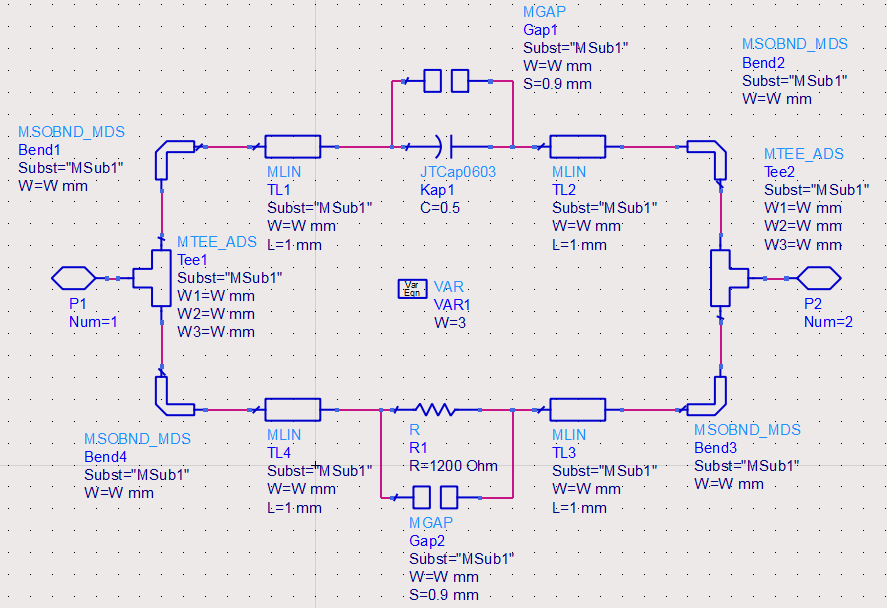
\includegraphics[width=0.8\textwidth]{img/Stabilization_circuit}
	  \caption{RC-filter for input stabilization}
	  \label{fig:Stabschem}
  \end{figure}

  \begin{figure}[H]
	  \begin{minipage}[b]{.45\textwidth}
	  \centering
	  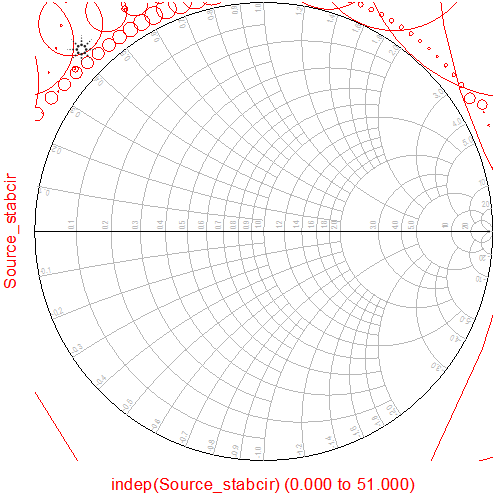
\includegraphics[width=\linewidth]{img/Stabilization_source_circle}
  	  \caption{Amplifier input stability circle}
	  \label{fig:Stabcircle_in}
  \end{minipage}%
  \begin{minipage}{.1\textwidth}
	  \hspace{\linewidth}
  \end{minipage}%
  \begin{minipage}[b]{.45\textwidth}
	  \centering
	  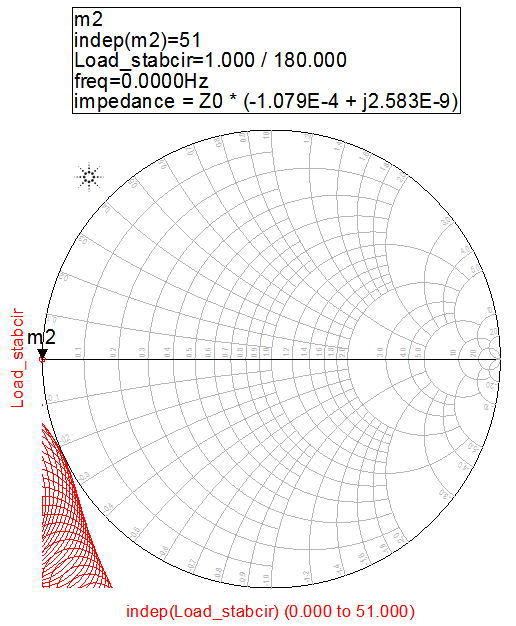
\includegraphics[width=\linewidth]{img/Stabilization_load_circle}
  	  \caption{Amplifier output stability circle}
	  \label{fig:Stabcircle_out}
  \end{minipage}
  \end{figure}

  \section{Bias network}

  The purpose of a bias network is to filter unwanted noise from the bias voltage sources to prevent it from reaching the gate and drain terminals, and to prevent RF signal from the amplifier input and output from reaching the bias voltage sources. We are using two identical bias networks for the gate and drain bias voltages, which is composed of a microstrip quarter-wave transformer which blocks the input or output signal from reaching the bias source, and a capacitor bank that filters out noise from the bias voltage sources.

  Figure~\ref{fig:Biasschem} shows the bias network we are using, with the probes used for measuring S-parameter characteristics. We have first simulated the two-port characteristics with terminal 1 at the input and terminal 2 at the point that will be connected to the transistor's gate or drain. Figure~\ref{fig:Biastwos} shows two-port parameters $S_1$$_2$ and $S_2$$_2$, which shows that within our designated frequency band from 2.35 to 2.45 GHz, only between -42 and -50 dB of the input signal gets transmitted to the bias voltage source.

  We have also simulated one-port S-parameters by grounding the input of the circuit and measuring the reflection coefficient at the output ($S_1$$_1$). This is more relevant to real-world conditions as the DC voltage source providing the bias voltage will act as an AC ground. The results of this simulation is shown in figure~\ref{fig:Biasones}. The simulation shows that within the 2.35-2.45 GHz band almost all of the incident wave is reflected, while we have a -6dB attenuation of the reflected incident wave at approx. 1.8 GHz.

  \clearpage


  \begin{figure}[h]
  	  \centering
	  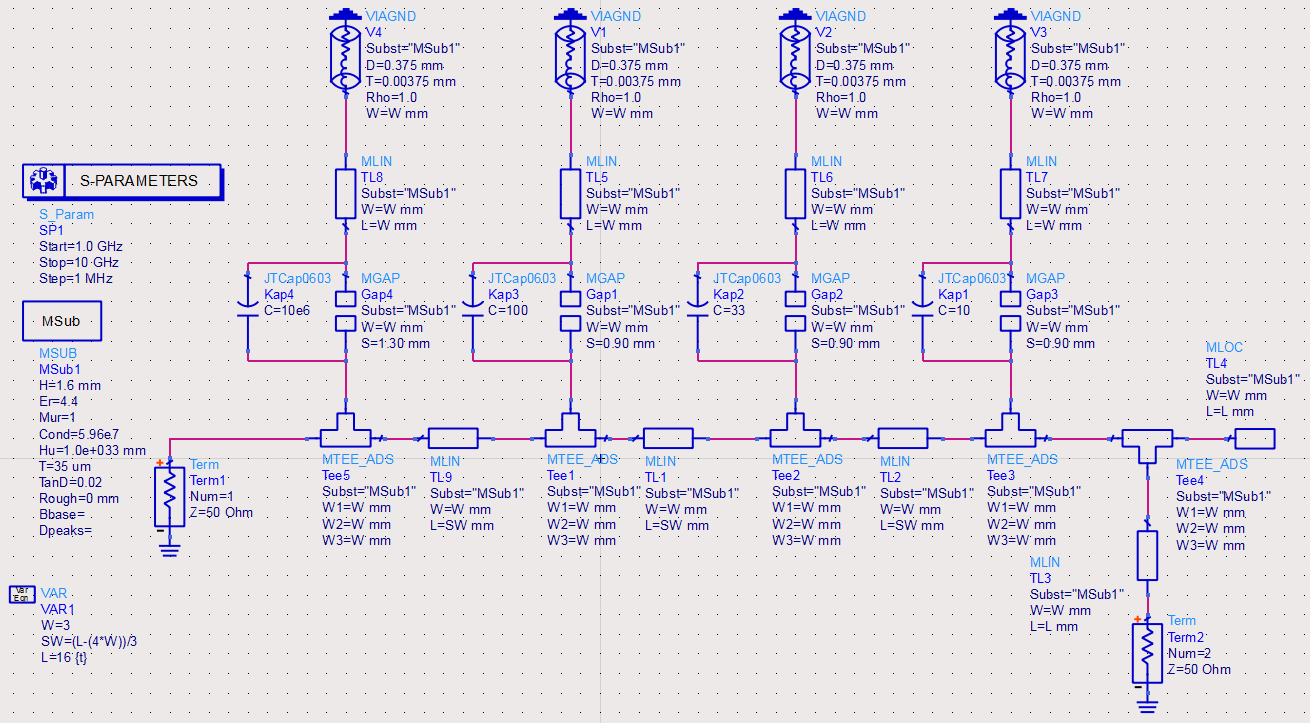
\includegraphics[width=\textwidth]{img/Bias_filter_two_port}
  	  \caption{Gate bias network schematics}
  	  \label{fig:Biasschem}
  \end{figure}

  \begin{figure}[h]
	  \begin{minipage}[b]{.45\textwidth}
	  \centering
	  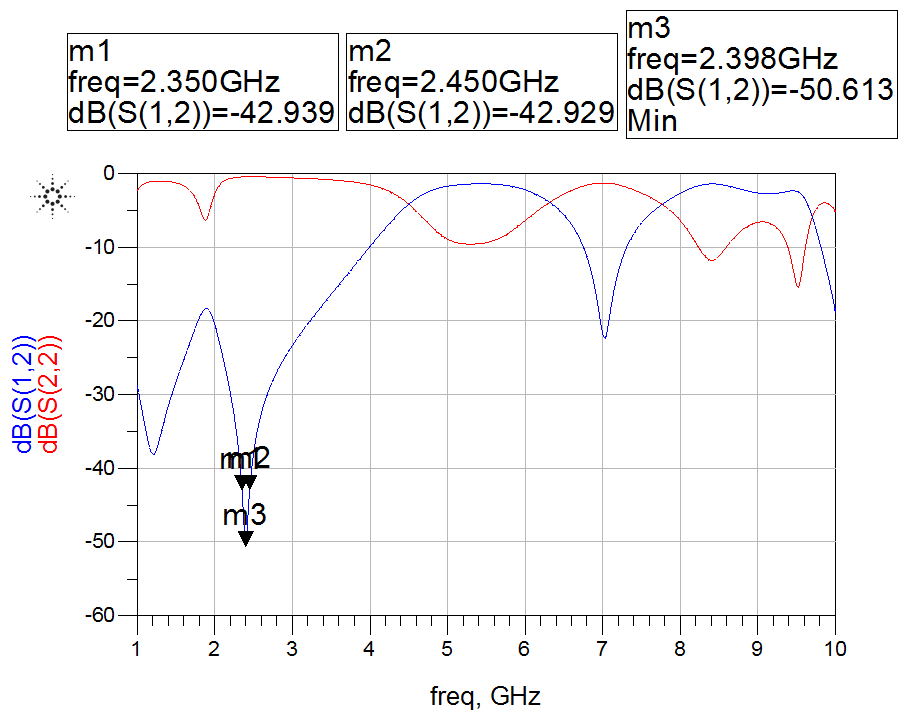
\includegraphics[width=\linewidth]{img/Bias_filter_two_port_s_parm}
	  \caption{Bias network two-port S-parameter}
  	  \label{fig:Biastwos}
  \end{minipage}%
  \begin{minipage}{.1\textwidth}
	  \hspace{\linewidth}
  \end{minipage}%
  \begin{minipage}[b]{.45\textwidth}
	  \centering
	  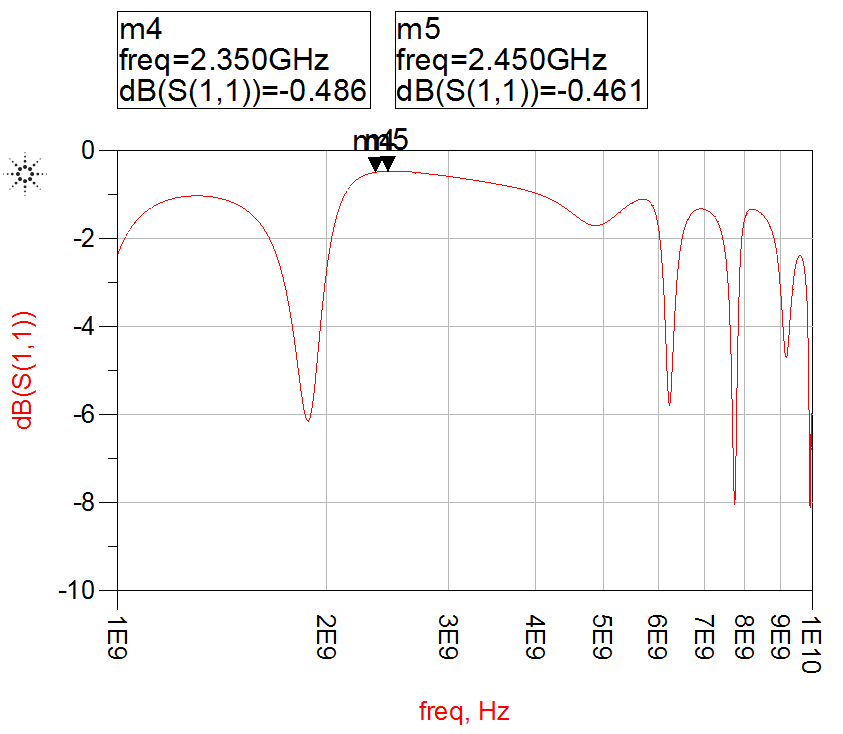
\includegraphics[width=\linewidth]{img/Bias_filter_one_port_s_parm}
  	  \caption{Bias network one-port S-parameter}
  	  \label{fig:Biasones}
  \end{minipage}
  \end{figure}


  \section{Matching network}
  Finally, to achieve the required gain specifications, the input and output of the amplifier should be impedance matched to as close as possible to $50 \Omega$. This is because the maximum power transfer occurs when both source and load have the same impedance. We are using series capacitors and shunt inductors at both input and output, which is beneficial since the series capacitors will double as DC blocking elements as well.

  \begin{figure}[h]
	  \centering
	  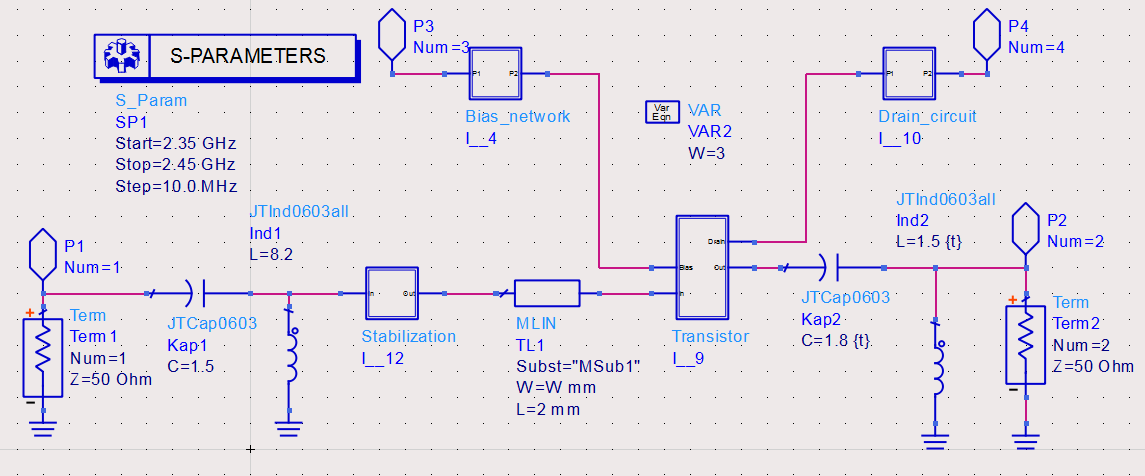
\includegraphics[width=\textwidth]{img/Matching_circuit}
	  \caption{Schematics of amplifier with matching network}
  	  \label{fig:Matchschem}
  \end{figure}

  \begin{figure}[h]
	  \begin{minipage}[b]{0.45\textwidth}
	  \centering
	  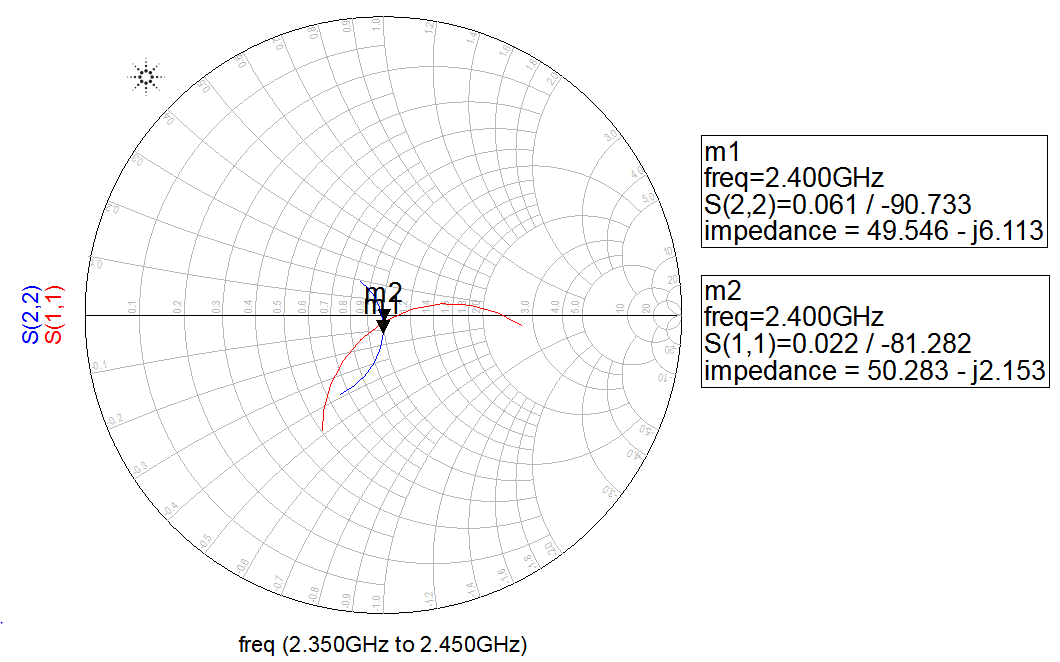
\includegraphics[width=\linewidth]{img/Matching_smith_chart}
  	  \caption{Input (red curve) and output (blue curve) impedances plotted for 2.35-2.45 GHz spectrum}
 	  \label{fig:MatchSmith}
  \end{minipage}%
  \begin{minipage}{.1\textwidth}
	  \hspace{\linewidth}
  \end{minipage}%
  \begin{minipage}[b]{0.45\textwidth}
	  \centering
	  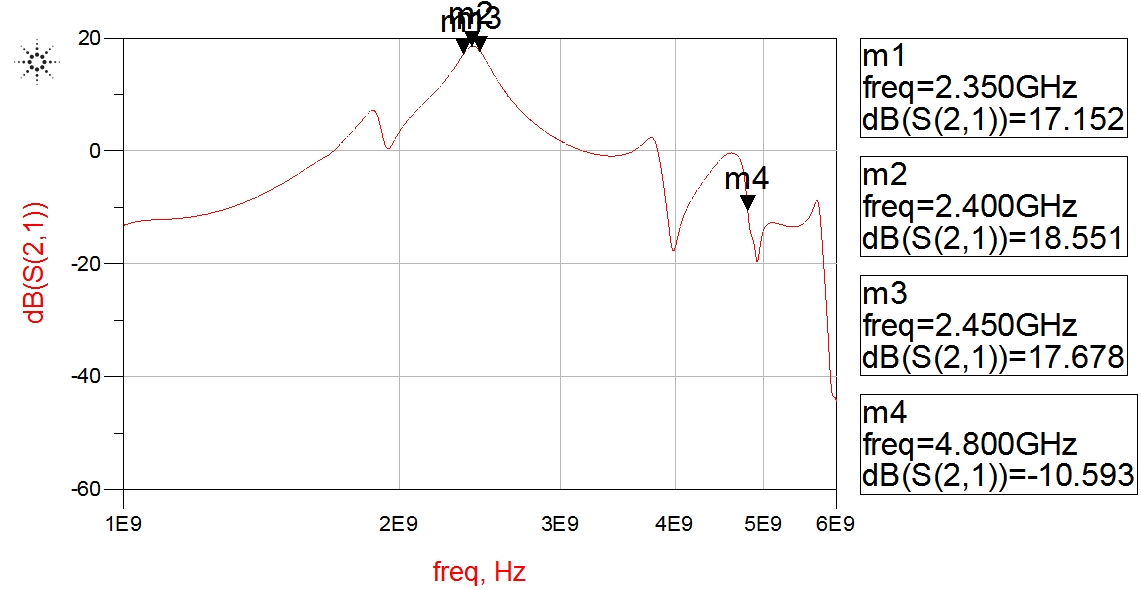
\includegraphics[width=\linewidth]{img/Small_signal_gain_matched}
  	  \caption{Gain figure for matched circuit}
  	  \label{fig:MatchGain}
  \end{minipage}
  \end{figure}


  \chapter{Results}

\section{Simulated results}
This section lists the results from the simulation done in the Keysight Advanced Design System (ADS) software suite.

\subsection{Transistor I-V curve}

  \begin{figure}[H]
	  \centering
	  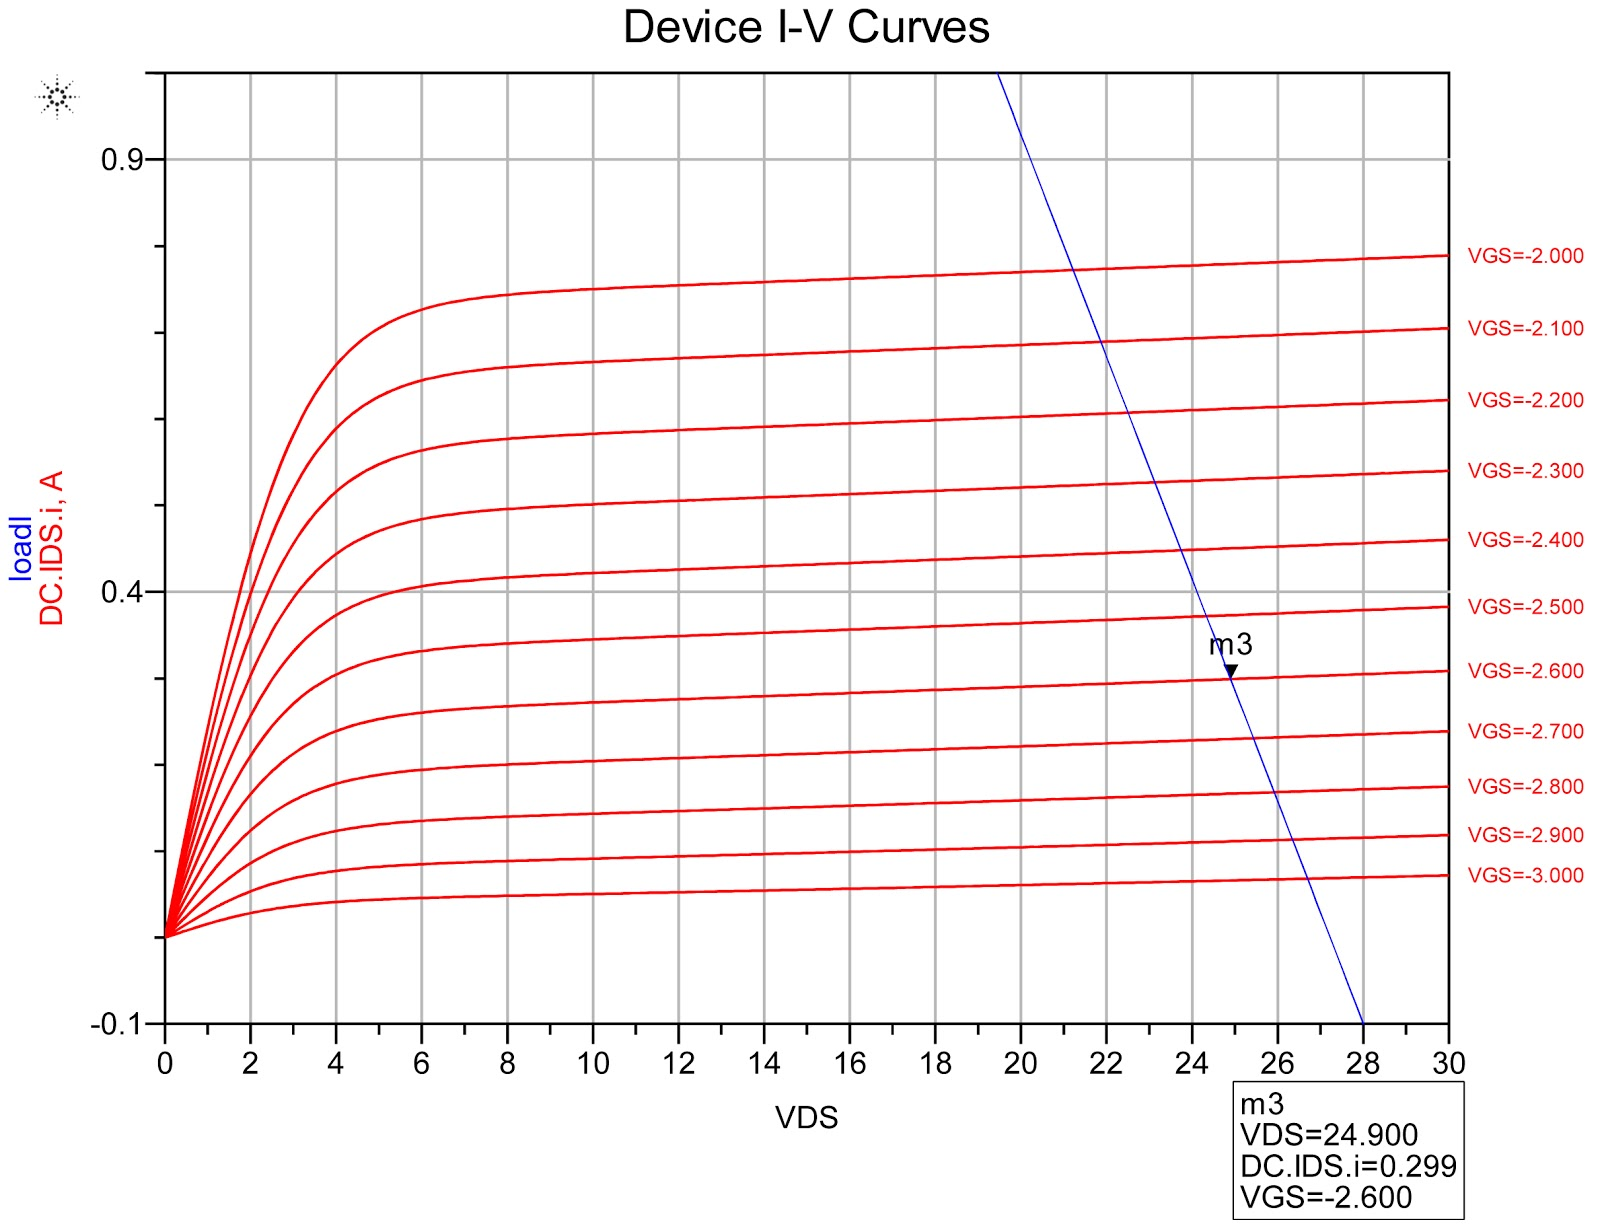
\includegraphics[width=0.75\textwidth]{img/01_IVCurve}
	  \caption{Simulated drain current for different drain and gate bias voltages with a load-line}
	  \label{fig:fig_IV}
  \end{figure}

  Note that the transistor model used is only valid for VDS voltages between 28 and 48 volts, meaning that the I-V-curves are at best approximate below 28 volts.

  \subsection{Stability simulations}

  \begin{figure}[H]
	  \begin{minipage}[b]{.45\textwidth}
	  \centering
	  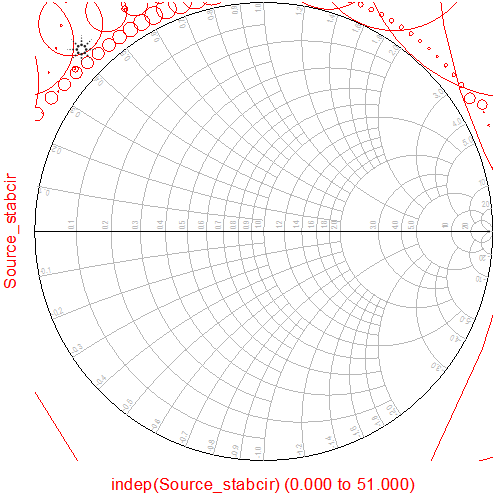
\includegraphics[width=\linewidth]{img/Stabilization_source_circle}
  	  %\caption{Amplifier input stability circle}
	  \label{fig:Stabcircle_in}
  \end{minipage}%
  \begin{minipage}{.1\textwidth}
	  \hspace{\linewidth}
  \end{minipage}%
  \begin{minipage}[b]{.45\textwidth}
	  \centering
	  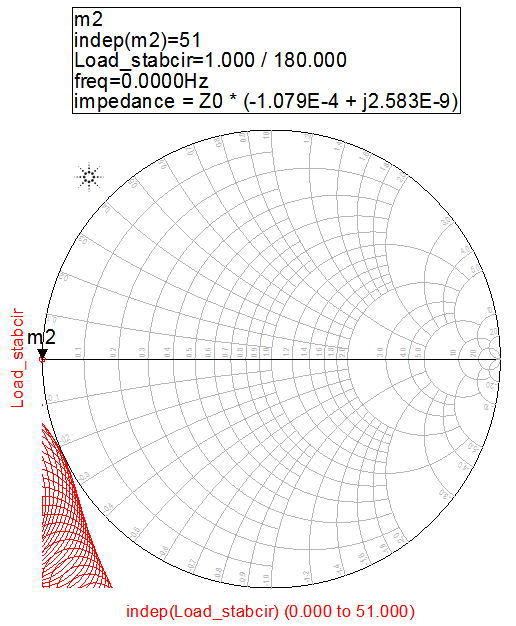
\includegraphics[width=\linewidth]{img/Stabilization_load_circle}
  	  %\caption{Amplifier output stability circle}
	  \label{fig:Stabcircle_out}
  \end{minipage}
  \caption{Smith-chart representation of the stability circles for source (left) and load (right) for frequencies between 0Hz and 6GHz}
  \label{fig:Stabcircle}
  \end{figure}

  \subsection{Small-signal gain}

  \begin{figure}[H]
	  \centering
	  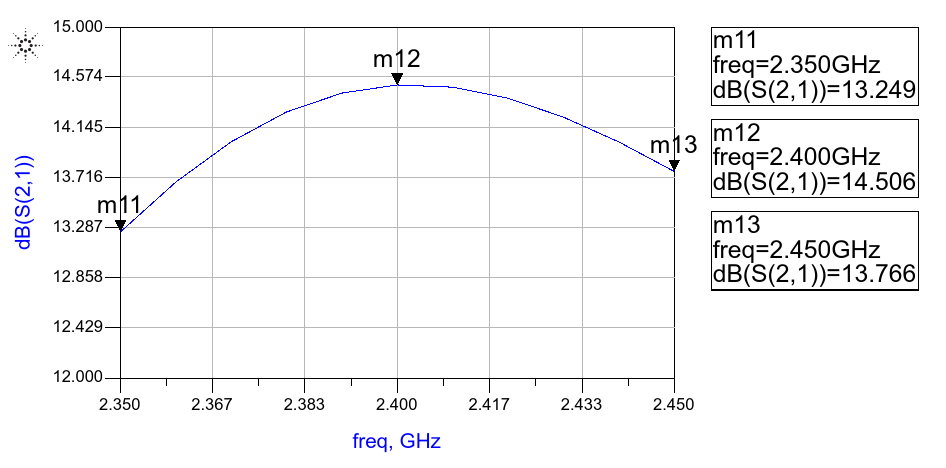
\includegraphics[width=0.75\textwidth]{img/Sim_S21}
	  \caption{Simulated small-signal gain within the band of operation}
	  \label{fig:Sim_S21}
  \end{figure}

  The small-signal gain ($S_{21}$) has a peak value of 14.506 dB at 2.4GHz, and a minimum value within the band of operations of 13.287 dB, giving a maximum variation of 1.257 dB within the 100MHz band of operation.

  \subsection{Large-signal gain}

  \begin{table}[H]
	  \centering
	  \begin{tabular}{l l l}
		  Frequency & Output power & gain \\
		  2.35 GHz & 38.71dBm & 11.71dB \\
		  2.40 GHz & 39.26dBm & 12.26dB \\
		  2.45 GHz & 38.87dBm & 11.87dB
	  \end{tabular}
	  \caption{Simulated output power with input power of 27dBm}
	  \label{tab:sim_power}
  \end{table}

  \subsection{Power added efficiency (PAE)}
  
  \begin{table}[H]
	  \centering
	  \begin{tabular}{l l}
		  Frequency & PAE \\
		  2.35 GHz & 40.30\% \\
		  2.40 GHz & 41.79\% \\
		  2.45 GHz & 42.59\%
	  \end{tabular}
	  \caption{Simulated power added efficiency with output power of 38dBm}
	  \label{tab:sim_pae}
  \end{table}

  \subsection{Third-order intermodulation distortion (TOIMD)}

  \begin{table}[H]
	  \centering
	  \begin{tabular}{l l}
		  TOIMD high & -15.35dBc \\
		  TOIMD low & -15.62dBc
	  \end{tabular}
	  \caption{Simulated third-order intermodulation distortion with output power of 38dBm}
	  \label{tab:sim_toimd}
  \end{table}

  \section{Measured results}
  This section lists the results from the measurements done on the real circuit in the laboratory.

  \subsection{Small-signal gain}

  \begin{figure}[H]
	  \centering
	  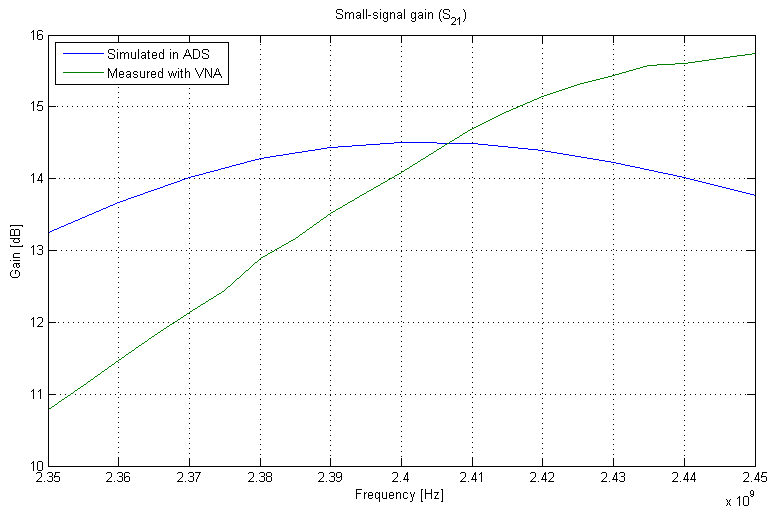
\includegraphics[width=0.75\textwidth]{img/S21_meas_sim}
	  \caption{Measured small-signal gain (green) compared to simulated small-signal gain (blue) within the band of operation}
	  \label{fig:Meas_S21}
  \end{figure}

Minimum measured gain was 10.79dB at 2.35 GHz, while the maximum was measured to 15.74dB at 2.45 GHz. At the center frequency of 2.40 GHz the small-signal gain was 14.08dB

  \subsection{Large-signal gain}

  \begin{figure}[h]
	  \centering
	  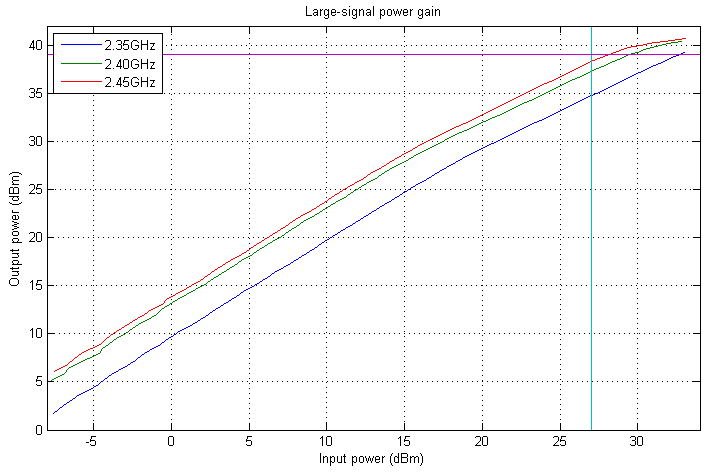
\includegraphics[width=0.75\textwidth]{img/Power_Out_1tone}
	  \caption{Measured output power at three different frequencies}
	  \label{fig:Meas_Pout}
  \end{figure}

  \begin{table}[H]
	  \centering
	  \begin{tabular}{l l l}
		  Frequency & Output power\\
		  2.35 GHz & 34.73dBm \\
		  2.40 GHz & 37.17dBm \\
		  2.45 GHz & 38.37dBm
	  \end{tabular}
	  \caption{Measured power output with an input power of 27dBm}
	  \label{tab:Meas_Pout}
  \end{table}

  \subsection{Power added efficiency (PAE)}

% \begin{figure}[H]
%	  \centering
%	  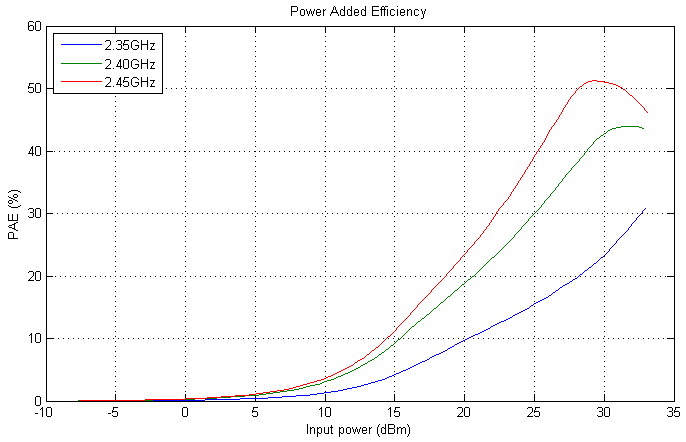
\includegraphics[width=0.75\textwidth]{img/Power_Added_Efficiency}
%	  \caption{Measured power added efficiency at three different frequencies}
%	  \label{fig:Meas_Pae}
%  \end{figure}

  \begin{table}[H]
	  \centering
	  \begin{tabular}{l l}
		  Frequency & PAE \\
		  2.35 GHz & 18.26\% \\
		  2.40 GHz & 35.02\% \\
		  2.45 GHz & 46.99\%
	  \end{tabular}
	  \caption{Measured power added efficiency with output power of 38dBm}
	  \label{tab:Meas_Pae}
  \end{table}

  \subsection{Third-order intermodulation distortion}

    \begin{table}[H]
	  \centering
	  \begin{tabular}{l l}
		  TOIMD high & -22.41dBc \\
		  TOIMD low & -22.45dBc
	  \end{tabular}
	  \caption{Measured third-order intermodulation distortion with output power of 38dBm}
	  \label{tab:Meas_Toimd}
  \end{table}

  \subsection{Summary of measured results}

  \begin{table}[H]
	  \centering
	  \begin{tabular}{p{4.5cm} | p{1.7cm} p{2.7cm} p{1.7cm} l}
		  Parameter & 2.35 GHz & 2.40 GHz & 2.45 GHz & Requirement \\
		  \hline
		  Small-signal gain & 10.79dB & 14.08dB & 15.74dB & $>13dB$ \\
		  Output power with 27dBm input & 34.73dBm & 37.17dBm & 38.37dBm & $>39dBm$ \\
		  Power added efficiency & 18.26\% & 35.02\% & 46.99\% & - \\
		  Third-order intermodulation distortion & & high: -22.41dBc low: -22.45dBc & & - \\
	  \end{tabular}
	  \caption{Summary of measured results}
	  \label{tab:Meas_Sum}
  \end{table}


    


  \chapter{Discussion}

  \section{Fulfillment of requirements}
	\subsection{Stability}
	The amplifier was simulated to be unconditionally stable for all frequencies at all source and load impedances except for when the output was presented with a short-circuit to ground. In real life, it was only tested with a $50 \Omega$ termination on the input and a $50 \Omega$ dummy load, for which it proved not to oscillate at any frequency seen on the spectrum analyzer. No tendencies to start oscillating was seen when doing both small- and large-signal testing. To our best knowledge, the requirement of stability was fulfilled.
	\subsection{Small-signal gain and bandwidth}
	The simulated gain was within the requirement specification with a minimum value of 13.287dBm across the 100 MHz bandwidth. The measured gain was below the required minimum of 13dBm for the frequency range of 2.35 - 2.38 GHz, while it was above the 13dBm limit for the rest of the band of operation. This requirement was hence not fulfilled.
	\subsection{Large-signal gain}
	For an input power of 27dBm, the required output power of 39dBm was not achieved at any of the tested frequencies of 2.35 GHz, 2.40 GHz and 2.45 GHz. This requirement was then not fulfilled.
  \section{Other results}
	\subsection{Power added efficiency}
	The power added efficiency exhibits the same shift in frequency as the gain, with the best performance at 2.45 GHz, while the results at 2.35 GHz and 2.40 GHz are below the results from the simulations in ADS. 
	\subsection{Third-order intermodulation distortion}
	The third-order intermodulation distortion (TOIMD) was measured to be below -22dBc for all output power levels up to 38dBm. This level of TOIMD is similar to what was achieved in a comparable amplifier design described in \cite{5WLTE}, which should mean that this is an acceptable TOIMD level, again indicating that the amplifier shows good linearity.
  \section{What happened}
  The shape of the measured small-signal gain curve shows that the maximum gain is not at our center frequency of 2.40 GHz where it was designed to be, but probably at or above 2.45GHz. This is most probably due to incorrect matching at the input or output. Since the center frequency was shifted upwards, this indicates that the electrical length of the matching network stubs is shorter than expected. This again leads to the observation that the propagation speed in the substrate is higher than expected, which must mean that the permittivity of the substrate is lower than expected.

  Variations in the relative permittivity of the substrate is not uncommon when using standard FR-4 substrate, as this type of substrate by nature has a highly variable permittivity. If absolute control of the permittivity of the substrate is required, special, more expensive RF substrate should be used.

  Since the small-signal gain at 2.45 GHz was well above the requirements, it is highly probable that the amplifier would meet the requirement specifications if some effort was put into tuning the input and output matching networks to have the input and output impedances matched as closely as possible to 50 Ohms.
  
  \section{What was learned}
  When making rf-circuit prototypes it would be wise to make stub traces longer than what is calculated. This allows for adjustments post production to compensate for variations in the substrate permittivity. 

  \section{Conclusion}
  The project was successful in designing an RF power amplifier that is unconditionally stable, shows quite good efficiency and linearity characteristics and is functional in amplifying RF frequency signals.

  The project was not able to meet all point of the requirement specifications, however, having identified the most probable reasons for not fulfilling the required performance characteristics, it is believed that only a minor redesign should be needed to be able to reach the given performance criterions.

  The project was successful in teaching the students participating in the group the techniques for designing, simulating, building and measuring an RF power amplifier.


  %\begin{appendices}
  \appendix

  \chapter{Schematics and layout}

  \begin{figure}[h]
	  \centering
	  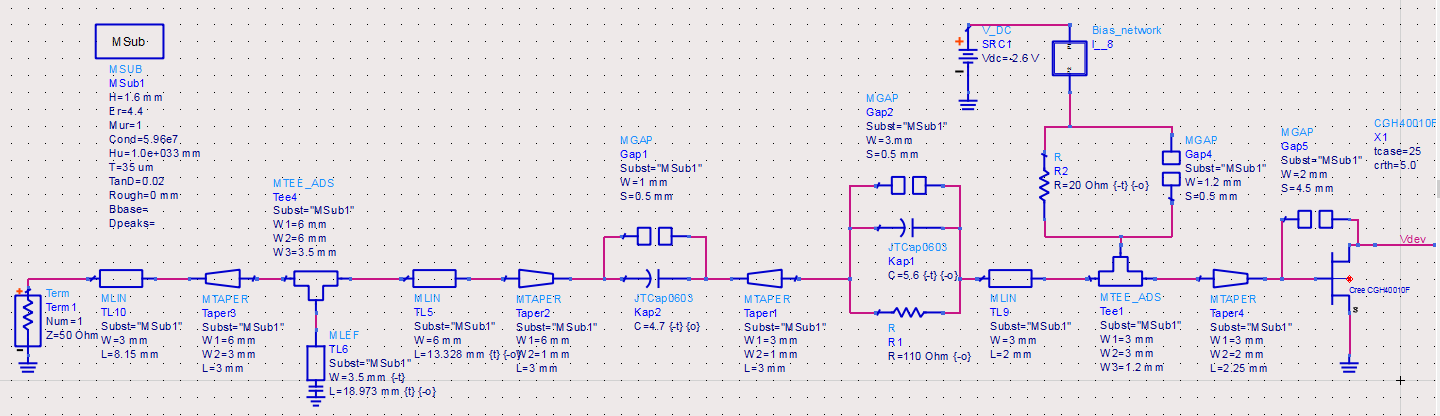
\includegraphics[width=\textwidth]{img/Circuit_input}
	  \caption{Input portion of amplifier circuit with S-parameter terminal}
	  \label{fig:Schem_Input}
  \end{figure}

  \begin{figure}[H]
	  \centering
	  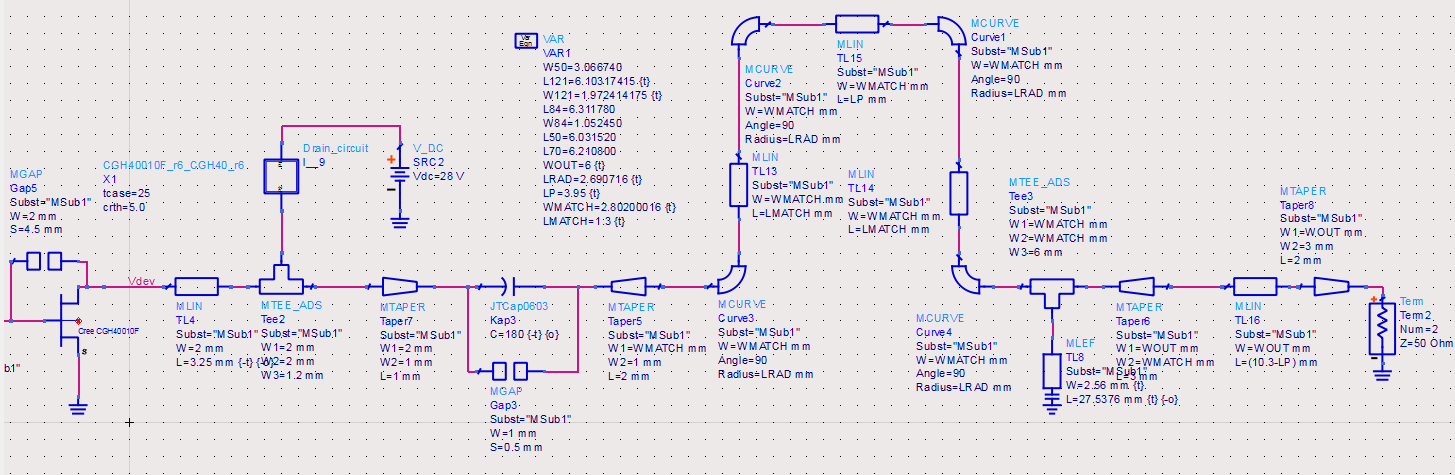
\includegraphics[width=\textwidth]{img/Circuit_output}
	  \caption{Output portion of amplifier circuit with S-parameter terminal}
	  \label{fig:Schem_Output}
  \end{figure}

  
  \begin{figure}[h]
	  \centering
	  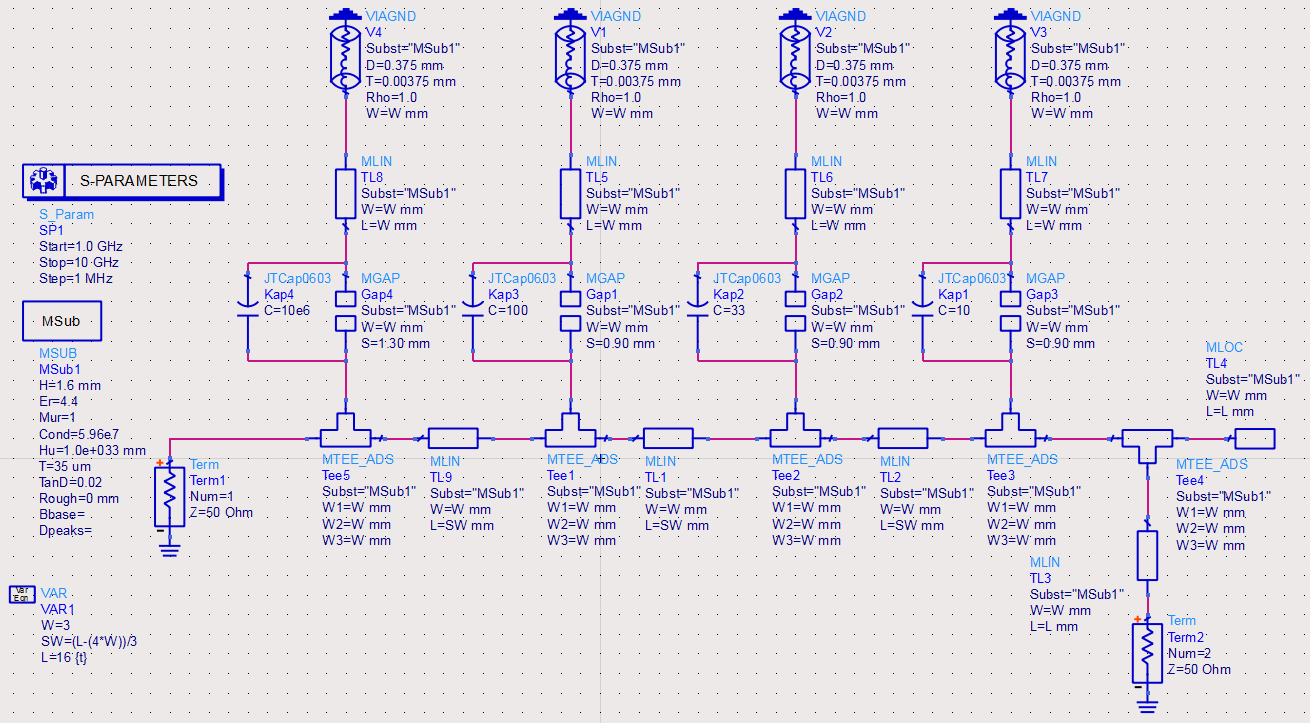
\includegraphics[width=\textwidth]{img/Bias_filter_two_port}
	  \caption{Schematics of input and output bias network}
	  \label{fig:Schem_Bias}
  \end{figure}

  \begin{figure}[h]
	  \centering
	  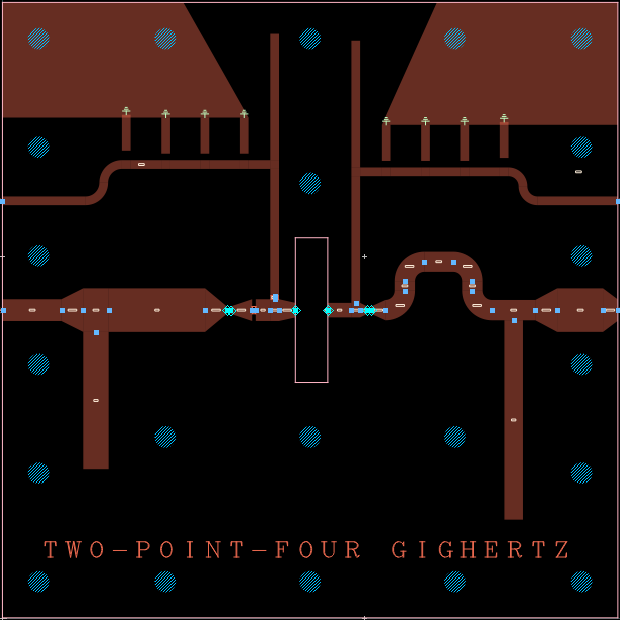
\includegraphics[width=0.75\textwidth]{img/Layout_ads}
	  \caption{PCB layout}
	  \label{fig:Layout}
  \end{figure}



\chapter{Additional graphs}

  \begin{figure}[h]
	  \centering
	  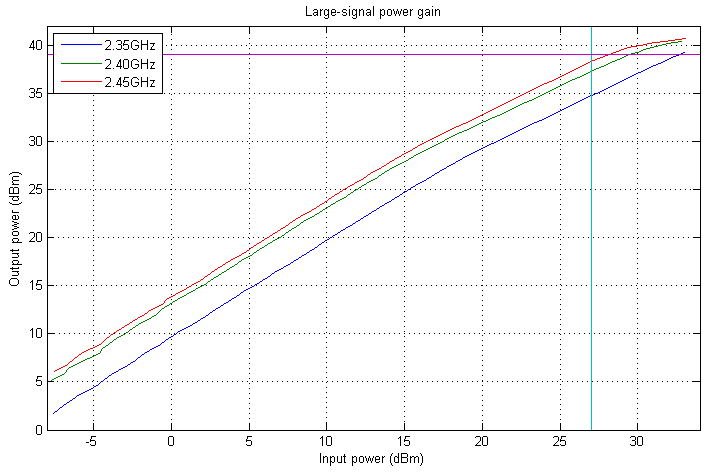
\includegraphics[width=0.75\textwidth]{img/Power_Out_1tone}
	  \caption{Measured output power at three different frequencies}
	  \label{fig:Meas_Pout}
  \end{figure}

  \begin{figure}[H]
	  \centering
	  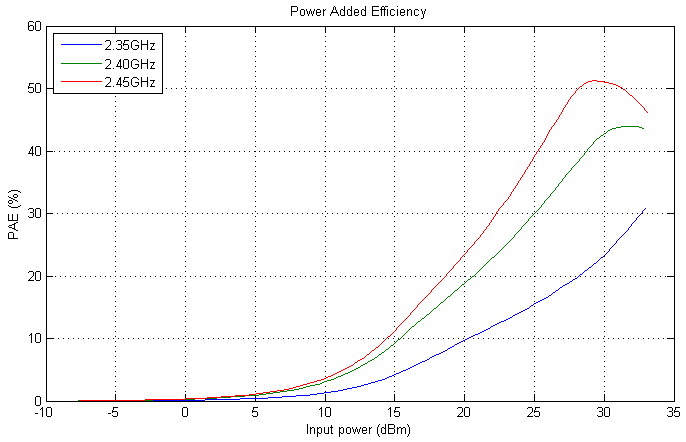
\includegraphics[width=0.75\textwidth]{img/Power_Added_Efficiency}
	  \caption{Measured power added efficiency at three different frequencies}
	  \label{fig:Meas_Pae}
  \end{figure}



  

  \begin{thebibliography}{9}

	  \bibitem{AmpRobertson}
		  I.D. Robertson, \emph{RFIC and MMIC Design and Technology}.
		  The Institution of Engineering and Technology,
		  2nd edition,
		  2001

  \end{thebibliography}

 
 % \end{appendices}
  
\end{document}
